\documentclass[10pt,a4paper]{article}	
\usepackage{amsmath}
\usepackage{amsfonts}
\usepackage{amssymb}
\usepackage{CJK}													% 支持中文
\usepackage{listings}											% 支持代码显示
\usepackage{color}												% 给文字,表格和图形上色(68种)
\usepackage{xcolor}												% color包的扩展
\usepackage[colorlinks,citecolor = blue, linkcolor=blue,hyperindex,CJKbookmarks]{hyperref}	% 链接功能
\usepackage{graphicx}											% 支持图片的插入
\usepackage{subfigure}											% 支持插入子图

%=============================c代码显示设置================================
%\lstset{
\lstdefinestyle{C}{
language=C,									% c语言
basicstyle=\small,							% 小号字体
numbers=left,								% 代码左边显行号
keywordstyle=\color{blue},					% 关键字用蓝色显示
numberstyle={\tiny\color{green}},			% 行号小小号,绿色	
numbersep=5pt,								% 行号与代码的距离
commentstyle=\small\color{red},				% 注释颜色和字号
backgroundcolor=\color[rgb]{0.95,1.0,1.0},	% 设置背景颜色
showspaces=false,							% 不显示空格
showtabs=false,								% 不显示\t
tabsize=4,									% \t的长短
frame=shadowbox, 							% 添加外框
framexleftmargin=5mm, 						% 外框左边的页边空白
rulesepcolor=\color{red!20!green!20!blue!20!},	%设置阴影颜色
breaklines=true,								% 自动断行
escapeinside=``,
extendedchars=false 							% 解决代码跨页时,章节标题,页眉等汉字不显示的问题
}
\lstdefinestyle{BASH}{
language=bash,								% bash代码
basicstyle=\small,							% 小号字体
numbers=left,								% 代码左边显行号
keywordstyle=\color{blue},					% 关键字用蓝色显示
numberstyle={\tiny\color{green}},			% 行号小小号,绿色	
numbersep=5pt,								% 行号与代码的距离
commentstyle=\small\color{red},				% 注释颜色和字号
backgroundcolor=\color[rgb]{1.0,0.95,1.0},	% 设置背景颜色
showspaces=false,							% 不显示空格
showtabs=false,								% 不显示\t
tabsize=4,									% \t的长短
frame=shadowbox, 							% 添加外框
framexleftmargin=5mm, 						% 外框左边的页边空白
rulesepcolor=\color{red!20!green!20!blue!20!},	%设置阴影颜色
breaklines=true,								% 自动断行
escapeinside=``,
extendedchars=false, 						% 解决代码跨页时,章节标题,页眉等汉字不显示的问题
morekeywords={cp,xz,tar,mount,umount,mkfs},
literate={\$}{{\textcolor{red}{\$}}}1
         {:}{{\textcolor{gray}{:}}}1
         {hjy@jy}{{\textcolor{orange}{hjy@jy}}}6
         {sudo}{{\textcolor{red}{sudo}}}4,
}
%========================================================================

\begin{document}

\begin{CJK*}{UTF8}{gkai}
%============================++题目和作者++================================
\title{ubuntu\thanks{ubuntu12.04LTS,64bit} 使用心得}					   						% 题目
\author{郝俊禹\thanks{Email:haojunyu2012@gmail.com}}				% 作者
%============================++++++++++++=================================
\date{}                                             				% 显示作者,不显示日期
\maketitle                                          				% 生成标题
\tableofcontents 												% 生成目录
\clearpage


%\part{内核}
%compile kernel
\section{编译内核}
\subsection{编译准备}
\begin{description}
\item[查看内核]	查看本机当前的内核版本\ref{fig:subfig1}--3.5.0.23-generic
\begin{lstlisting}[style=BASH]
hjy@jy:~$ uname -r
\end{lstlisting}
\begin{figure}[!htbp]
	\centering
	\caption{当前内核情况}
	\subfigure[本机当前的内核版本]{
		\label{fig:subfig1:a}
    		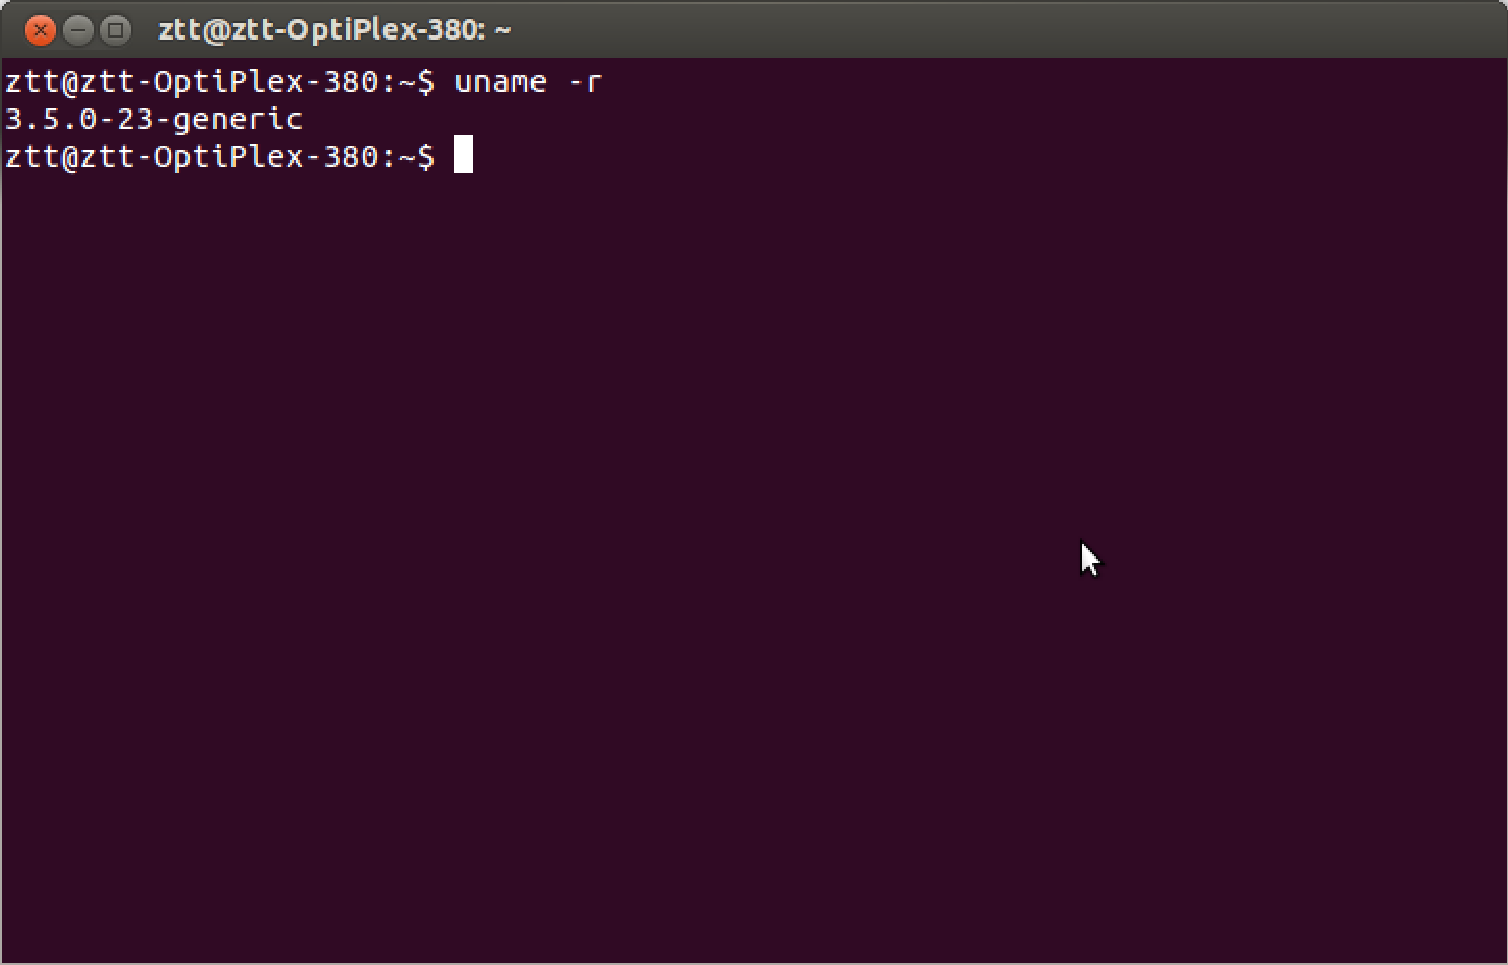
\includegraphics[scale=0.4]{figs/1.pdf}}
    	\subfigure[boot目录下文件]{
    		\label{fig:subfig1:b}
    		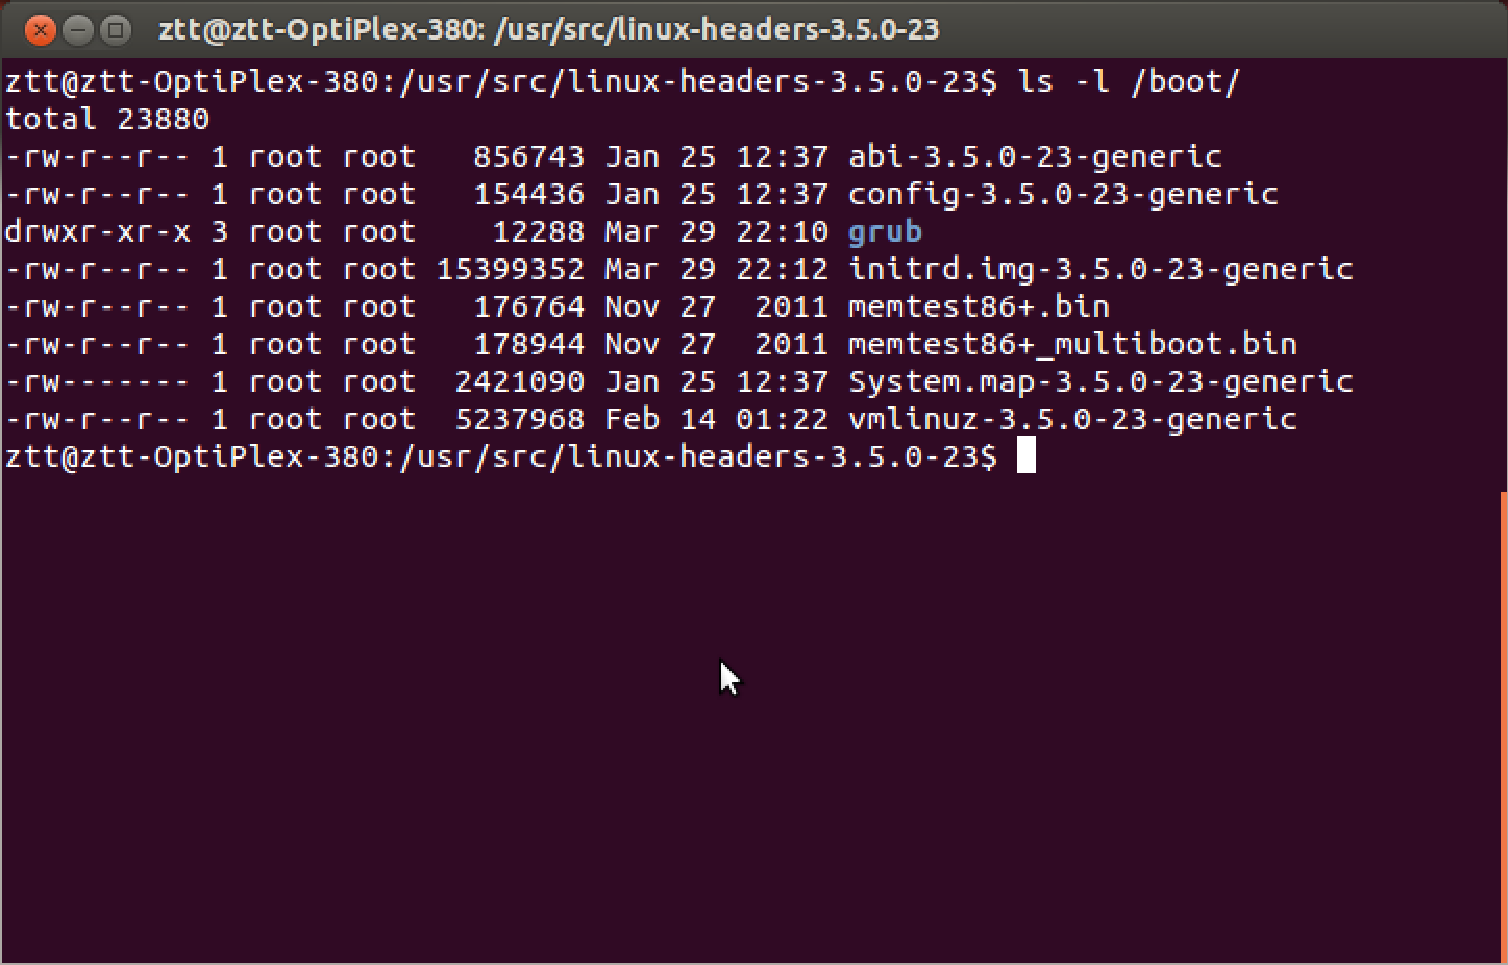
\includegraphics[scale=0.4]{figs/2.pdf}}
    	\label{fig:subfig1}
\end{figure}

\item[下载内核]	\href{http://www.kernel.org}{linux内核官网},建议下载stable的版本--linux-3.8.5.tar.xz

\item[拷贝文件]	将内核文件拷贝到/usr/src目录下.
\begin{lstlisting}[style=BASH]
hjy@jy:~$ sudo cp ~/Downloads/linux-3.8.5.tar.xz /usr/src
\end{lstlisting}

\item[解压文件]	解压.xz格式的文件要用xz\footnote{压缩:xz -z file.tar \& 解压:xz -d file.tar.xz} 命令
\begin{lstlisting}[style=BASH]
hjy@jy:~$ cd /usr/src
hjy@jy:/usr/src$ sudo xz -d linux-3.8.5.tar.xz
hjy@jy:/usr/src$ sudo tar -xvf linux-3.8.5.tar
\end{lstlisting}

\item[清理残留文件]	本步针对已经编译过多次的内核文件.如果是刚刚解开的包,不需要执行这一步
\begin{lstlisting}[style=BASH]
hjy@jy:/usr/src$ cd linux-3.8.5
hjy@jy:/usr/src/linux-3.8.5$ sudo make mrproper
\end{lstlisting}
\end{description}


\subsection{配置内核}
通过图形界面配置\footnote{参考网址:\url{http://forum.ubuntu.org.cn/viewtopic.php?t=134404} \& \url{http://lamp.linux.gov.cn/Linux/kernel_options.html}}
\begin{lstlisting}[style=BASH]
hjy@jy:/usr/src/linux-3.8.5$ sudo make menuconfig
\end{lstlisting}

\underline{\textit{可能出现的错误}:}
\begin{itemize}
\item requires the ncurses libraries.
\begin{lstlisting}[style=BASH]
hjy@jy:/usr/src/linux-3.8.5$ sudo apt-get install libncurses-dev
\end{lstlisting}
\end{itemize}

\begin{itemize}
\item General Setep
\begin{description}
\item[Prompt for development and/or incomplete code/drivers]	如果你的硬件比较新,那几乎是必须选的,这样,我们才可以找到4965无线网卡,alsa声音驱动等等。

\item[Kernel log buffer size]	我选15,双核。如果你用ia64,要选16。

\item[Control Group support]		集群支持?可以不要

\item[Choose SLAB allocator (SLUB (Unqueued Allocator))]	 内存管理模式选择slub
\end{description}


\item Block Layer
\begin{description}
\item[Support for Large Block Devices]	假如没有2TB的硬盘,就去掉

\item[Support for Large Single Files]	也不需要,谁有2TB的文件
\end{description}


\item \underline{Processor type and features}
\begin{description}
\item[Symmetric multi-processing support]	打开多核的开关,cpu是双核的,选中。

\item[Processor family (Core 2/newer Xeon)]	我的是Core 2/newer Xeon。

\item[Generic x86 support]	找到自己的cpu后,把选项去掉。

\item[Subarchitecture Type]	选(PC-compatible)

\item[Maximum number of CPUs]	输入自己的核心数目,我输入2

\item[SMT (Hyperthreading) scheduler support]	超线程技术,P4有支持的,我的t8100不支持,目前大部分市场上的家用cpu都不支持。

\item[High Memory Support (4GB)]	1G以下选1G;我是3G,选4G;4G以上的选16G

\item[Timer frequency]	默认是250Hz,较新的cpu都可以选择了1000Hz,性能更好。
\end{description}


\item Power Management Options
\begin{description}
\item[APM (Advanced Power Management) BIOS support]	现在的电脑都用acpi,去掉

\item[Default CPUFreq governor (conservative)]	cpu节电模式有四个,笔记本默认选conservative比较好。

\item[ACPI Processor P-States driver]	必须选,不然CPU Frequency就不能用。
\end{description}


\item Bus Options
\begin{description}
\item[网卡]	除了我的千兆网卡 Broadcom Tigon3 support和4965无线网卡Intel Wireless WiFi 4965AGN,其余的硬件支持统统去掉。

\item[声卡]	我的是hd声卡,我只是在PCI devices中,选intel hd 声卡,再选Build IDT/Sigmatel HD-audio codec support,除此之外的硬件支持全部去掉。

\item[SCSI device support]	现在都是SATA硬盘,一定要选*

\item[NatSemi SCx200 support]	去掉

\item[Support for PCI Hotplug (EXPERIMENTAL)]	如果没有PCI热插拔设备,去掉.这里的选项可以考虑全部编译进内核,而不是以模块形式存在。
\end{description}


\item \underline{Device Drivers}
\begin{description}
\item[PCI Express support]	现在新买的机器基本上都是PCI Express了

\item[SCSI disk support]		如果你的/boot放在SATA硬盘上,一定要选*。

\item[SCSI CDROM support]	用刻录机,必须选。
\end{description}


\item File Systems
\begin{description}
\item[Filesystem in Userspace support]	是必选的,如果你要用windows分区。

\item[ISO 9660 CDROM file system support]	一般选*

\item[VFAT (Windows-95) fs support]	 有FAT32分区就选*吧

\item[NTFS file system support]	有NTFS分区就选*吧

\item[NTFS write support]	如果想对 NTFS分区进行写操作,选*
\end{description}
\end{itemize}



\subsection{编译内核}
\begin{description}
\item[专用工具]	ubuntu编译内核的工具是make-kpkg,与其他的发行版相比,步骤相对简单.
\begin{lstlisting}[style=BASH]
hjy@jy:/usr/src/linux-3.8.5$ sudo make-kpkg clean
hjy@jy:/usr/src/linux-3.8.5$ sudo make-kpkg -initrd --append-to-version=hjy20130330 kernel_image kernel-headers
\end{lstlisting}

\underline{\textit{可能出现的错误}:}
\begin{itemize}
\item make-kpkg: command not found.
\begin{lstlisting}[style=BASH]
hjy@jy:/usr/src/linux-3.8.5$ sudo apt-get install kernel-package
\end{lstlisting}
\end{itemize}
\end{description}


\subsection{安装内核}
编译完成就是安装工作。编译好的内核在上一层目录。包括linux-headers-...-_i386.deb和linux-image-...-i386.deb两个文件,如果你不搞开发的话,只要安装内核就可以,头文件以后要用的时候再说。
\begin{lstlisting}[style=BASH]
hjy@jy:/usr/src/linux-3.8.5$ cd ..
hjy@jy:/usr/src/$ sudo dpkg -i linux-image-3.8.5+[tab]
\end{lstlisting}


\subsection{重启验证}
\begin{lstlisting}[style=BASH]
hjy@jy:/usr/src/$ sudo reboot
\end{lstlisting}
验证结果\ref{fig:subfig2}
\begin{figure}[!htbp]
	\centering
	\caption{升级内核后}
		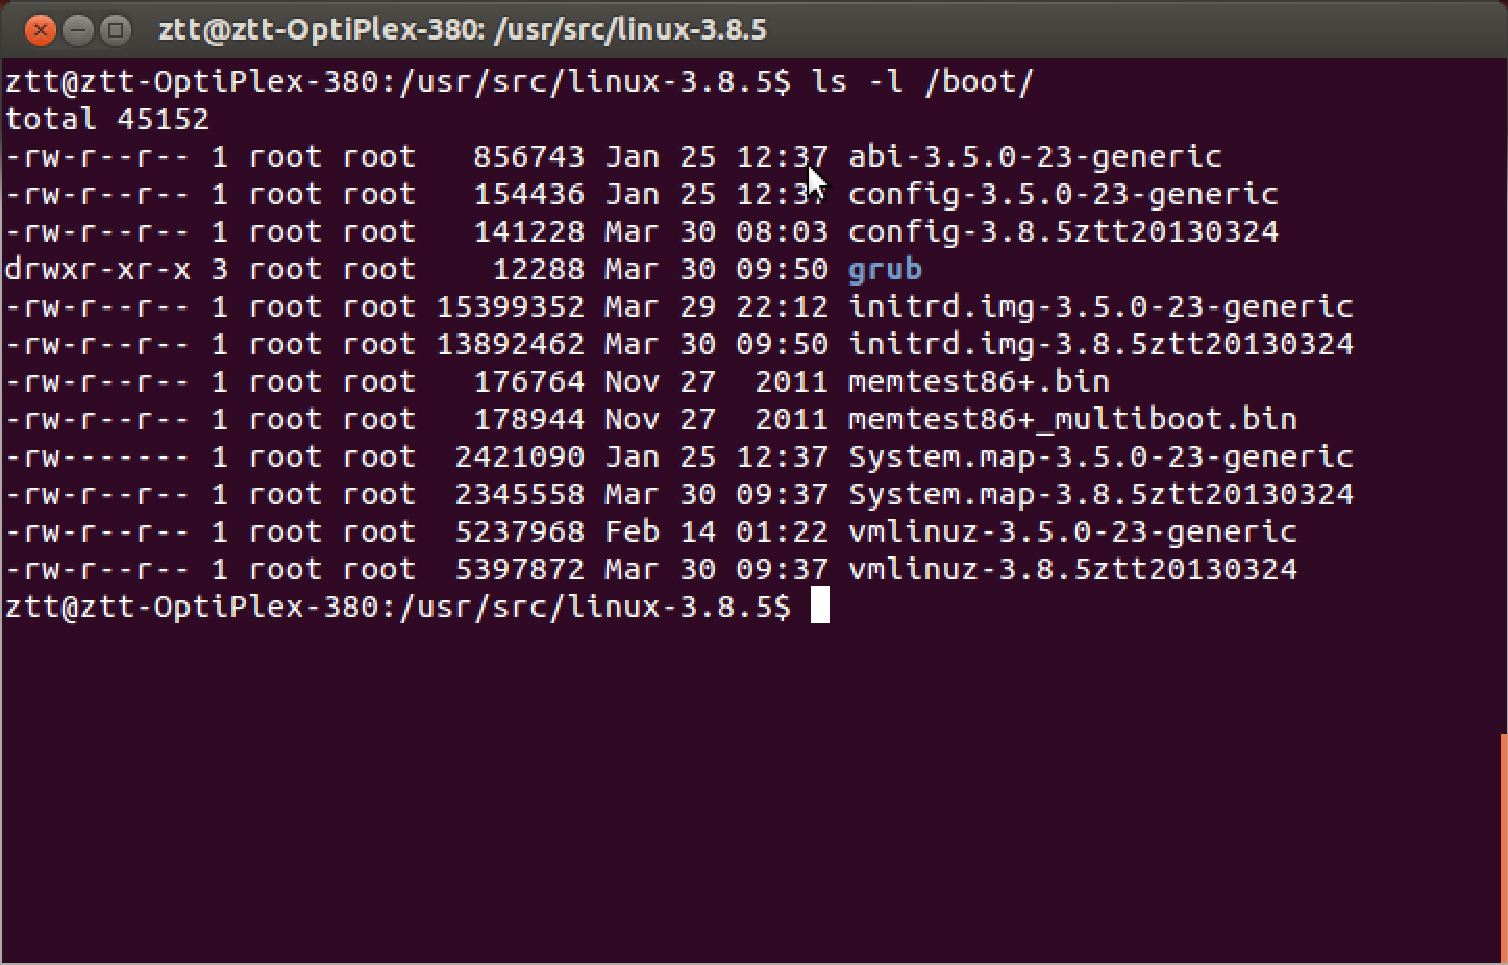
\includegraphics[scale=0.4]{figs/3.pdf}}
    	\label{fig:subfig2}
\end{figure}
\subsection{AFQ}
\subsubsection{准备}
\begin{enumerate}
\item 编译的内核与机器使用的多少位操作系统有关否?\\
答:无关

\end{enumerate}

\clearpage
%\documentclass[10pt,a4paper]{article}	
\usepackage{amsmath}
\usepackage{amsfonts}
\usepackage{amssymb}
\usepackage{CJK}													% 支持中文
\usepackage{listings}											% 支持代码显示
\usepackage{color}												% 给文字,表格和图形上色(68种)
\usepackage{xcolor}												% color包的扩展
\usepackage[colorlinks,citecolor = blue, linkcolor=blue,hyperindex,CJKbookmarks]{hyperref}	% 链接功能
\usepackage{graphicx}											% 支持图片的插入
%\usepackage{subfigure}											% 支持插入子图


%\lstset{
\lstdefinestyle{C}{
language=C,									% c语言
basicstyle=\small,							% 小号字体
numbers=left,								% 代码左边显行号
keywordstyle=\color{blue},					% 关键字用蓝色显示
numberstyle={\tiny\color{green}},			% 行号小小号,绿色	
numbersep=5pt,								% 行号与代码的距离
commentstyle=\small\color{red},				% 注释颜色和字号
backgroundcolor=\color[rgb]{0.95,1.0,1.0},	% 设置背景颜色
showspaces=false,							% 不显示空格
showtabs=false,								% 不显示\t
tabsize=4,									% \t的长短
frame=shadowbox, 							% 添加外框
framexleftmargin=5mm, 						% 外框左边的页边空白
rulesepcolor=\color{red!20!green!20!blue!20!},	%设置阴影颜色
breaklines=true,								% 自动断行
escapeinside=``,
extendedchars=false 							% 解决代码跨页时,章节标题,页眉等汉字不显示的问题
}
%=============================BASH代码显示设置================================
\lstdefinestyle{BASH}{
language=bash,								% bash代码
basicstyle=\small,							% 小号字体
numbers=left,								% 代码左边显行号
keywordstyle=\color{blue},					% 关键字用蓝色显示
numberstyle={\tiny\color{green}},			% 行号小小号,绿色	
numbersep=5pt,								% 行号与代码的距离
commentstyle=\small\color{red},				% 注释颜色和字号
backgroundcolor=\color[rgb]{1.0,0.95,1.0},	% 设置背景颜色
showspaces=false,							% 不显示空格
showtabs=false,								% 不显示\t
tabsize=4,									% \t的长短
frame=shadowbox, 							% 添加外框
framexleftmargin=5mm, 						% 外框左边的页边空白
rulesepcolor=\color{red!20!green!20!blue!20!},	%设置阴影颜色
breaklines=true,								% 自动断行
escapeinside=``,
extendedchars=false, 						% 解决代码跨页时,章节标题,页眉等汉字不显示的问题
morekeywords={cp,xz,tar,mount,umount,mkfs,git,ssh},
literate={\$}{{\textcolor{red}{\$}}}1
         {:}{{\textcolor{gray}{:}}}1
         {hjy@jy}{{\textcolor{orange}{hjy@jy}}}6
         {sudo}{{\textcolor{red}{sudo}}}4,
}
%========================================================================

\begin{document}

\begin{CJK*}{UTF8}{gkai}
%============================++题目和作者++================================
\title{实用软件推荐}						   						% 题目
\author{郝俊禹\thanks{Email:haojunyu2012@gmail.com}}				% 作者
%============================++++++++++++=================================
\date{}                                             				% 显示作者,不显示日期
\maketitle                                          				% 生成标题
\tableofcontents 												% 生成目录
\clearpage


\part{Windows}
\setcounter{section}{0}
\clearpage
\section{压缩刻录}


\section{聊天工具}
\section{视频软件}
\section{音乐软件}
\section{游戏软件}
\section{网络游戏}
\section{浏览器}
\section{图形图像}
\section{输入法}
\section{下载工具}
\section{办公软件}
\section{阅读翻译}
\clearpage
\section{系统工具}
\subsection{lmtghost3.0.exe-备份还原操作系统}
准备工作
\begin{itemize}
\item 备份还原软件--\href{http://ghost.laomaotao.net/help/330/}{老毛桃一键还原}
\end{itemize} 
操作步骤
\begin{itemize}
\item 备份系统
\begin{enumerate}
\item 主程序兼容Win2003、Winxp、Win7以及WinPE系统。为避免部分杀毒软件误报,请尽量在运行程序前退出杀软或在安全类软件提示是否允许操作时信任本程序运行。初次运行程序会提示进行初始备份,点击一键备份系统按钮后根据程序提示选择重新启动。\\
\begin{figure}[!htbp]
	\centering
	\caption{备份参数设置}  
		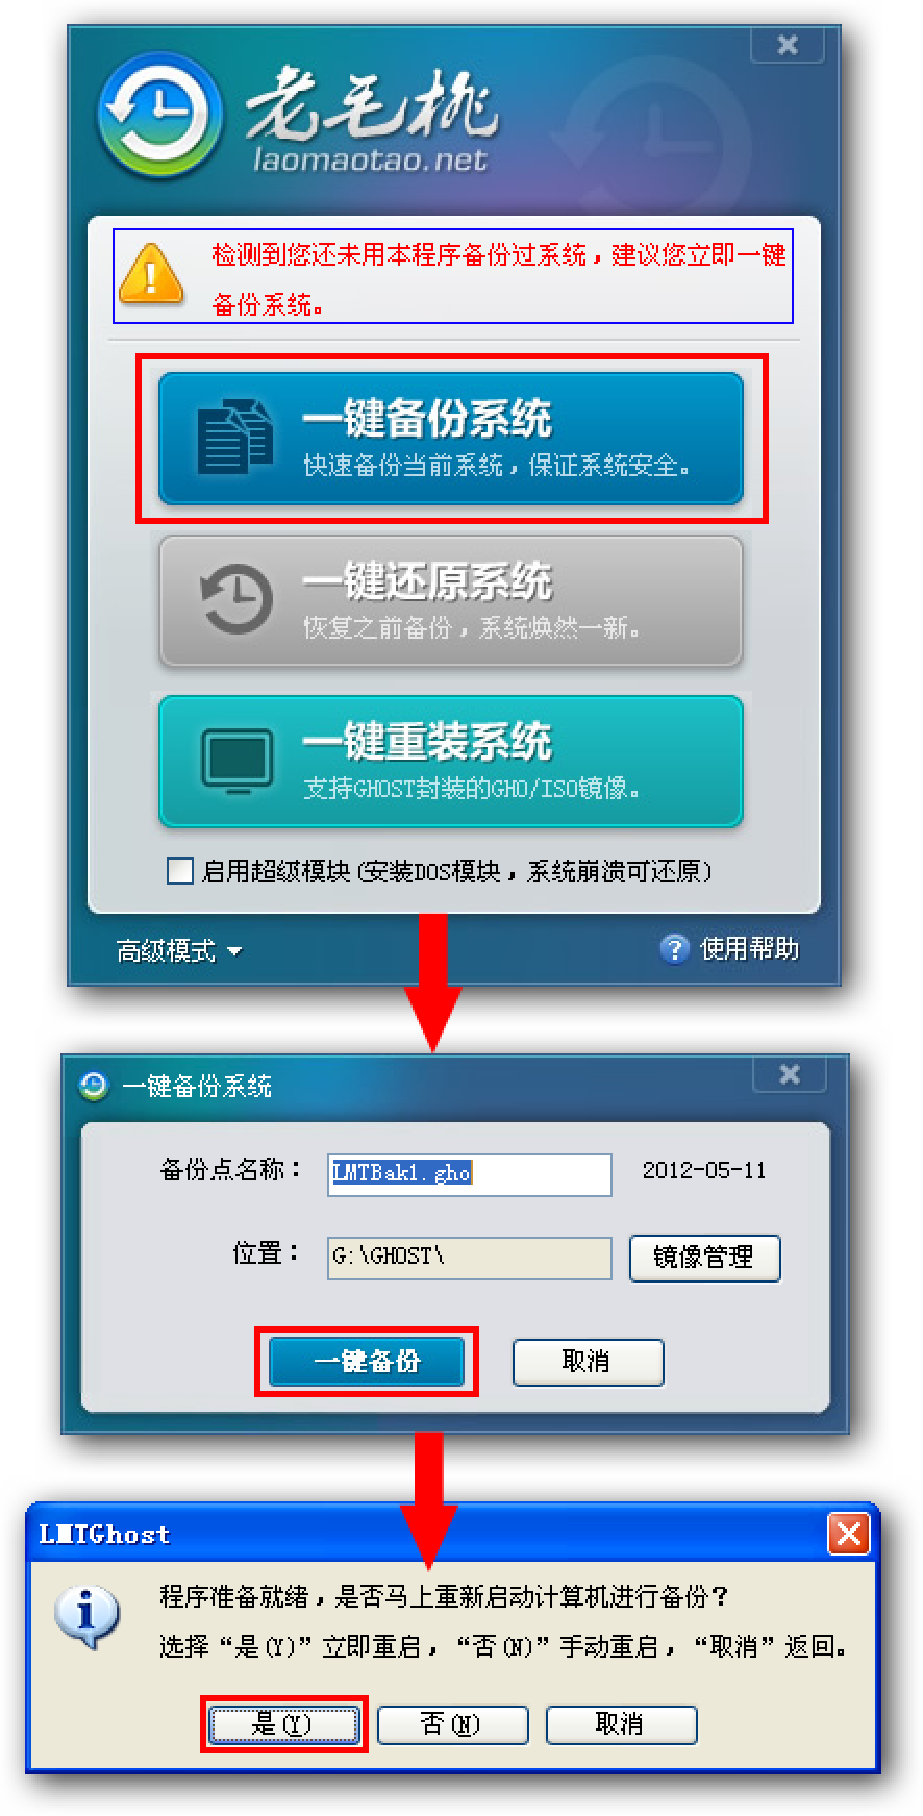
\includegraphics[scale=0.40]{figs/win_lmt_backup_startup.pdf}
    	\label{fig:win_lmt_backup_startup}
\end{figure}

\item 重新启动电脑后会自动进入老毛桃一键还原界面进行自动系统备份。\\
\begin{figure}[!htbp]
	\centering
	\caption{备份过程}  
		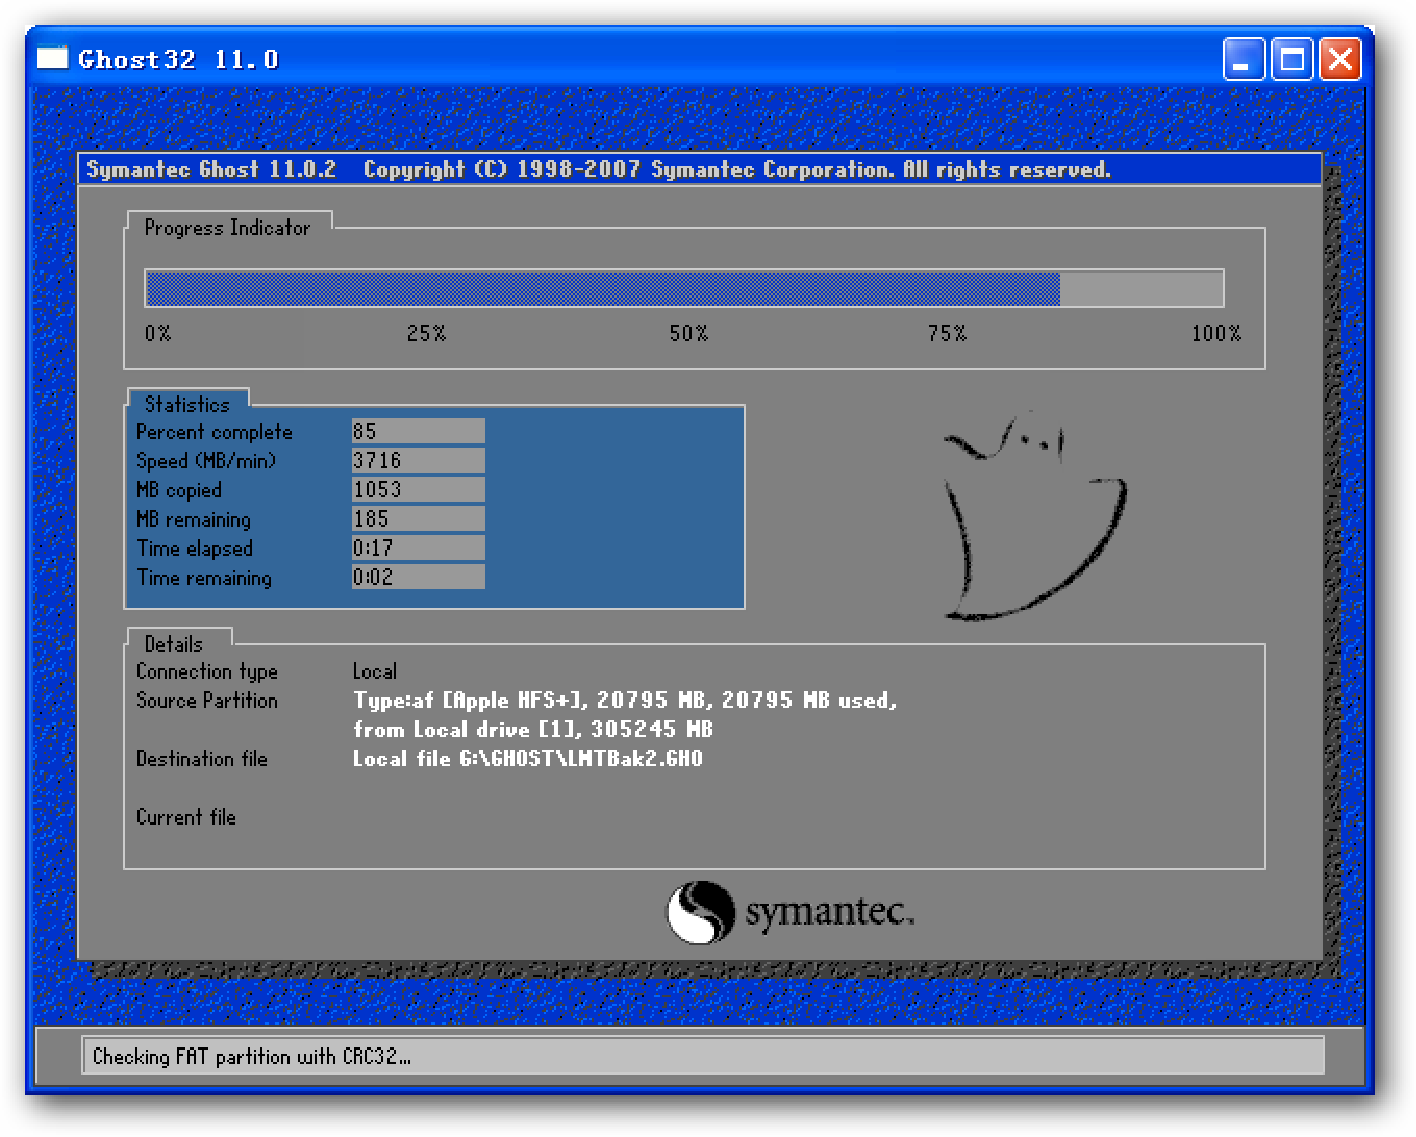
\includegraphics[scale=0.35]{figs/win_lmt_backup_set.pdf}
    	\label{fig:win_lmt_backup_set}
\end{figure}

\end{enumerate}

\item 还原系统\\
\begin{enumerate}
\item 备份完毕后重新启动电脑,打开老毛桃一键还原程序即可看到程序自动检测到刚刚备份了系统。以后当系统中毒或是出现其它问题时点击\textcolor{red}{(请在还原之前提前备份好系统盘的个人资料,还原时将对C盘原有数据进行覆盖)}。即可将系统恢复到之前备份的状态。\\
\begin{figure}[!htbp]
	\centering
	\caption{还原设置}  
		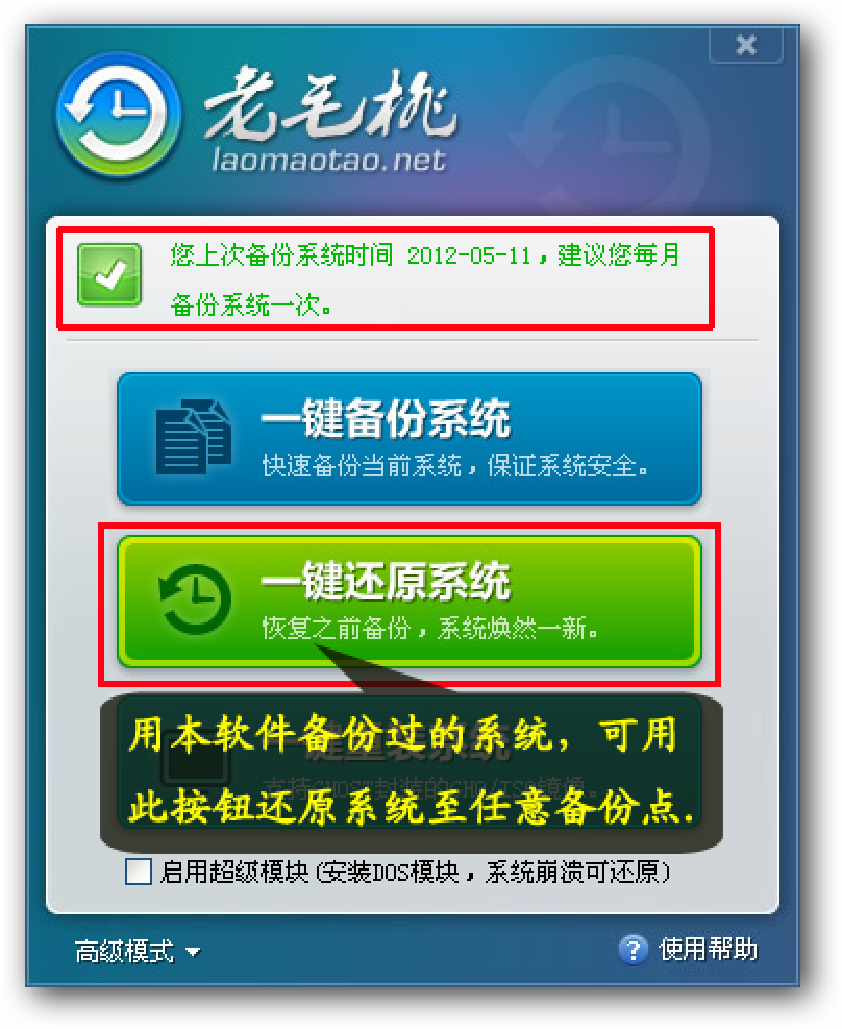
\includegraphics[scale=0.35]{figs/win_lmt_restore_startup.pdf}
    	\label{fig:win_lmt_backup_result}
\end{figure}
\end{enumerate}

\item 重装系统\\
\begin{enumerate}
\item 如果没有执行过系统备份想要重新安装系统,可以使用一键重装功能全新安装系统。一键重装系统功能支持GHOST封装的GHO/ISO镜像。\\
\begin{figure}[!htbp]
	\centering
	\caption{重装系统}  
		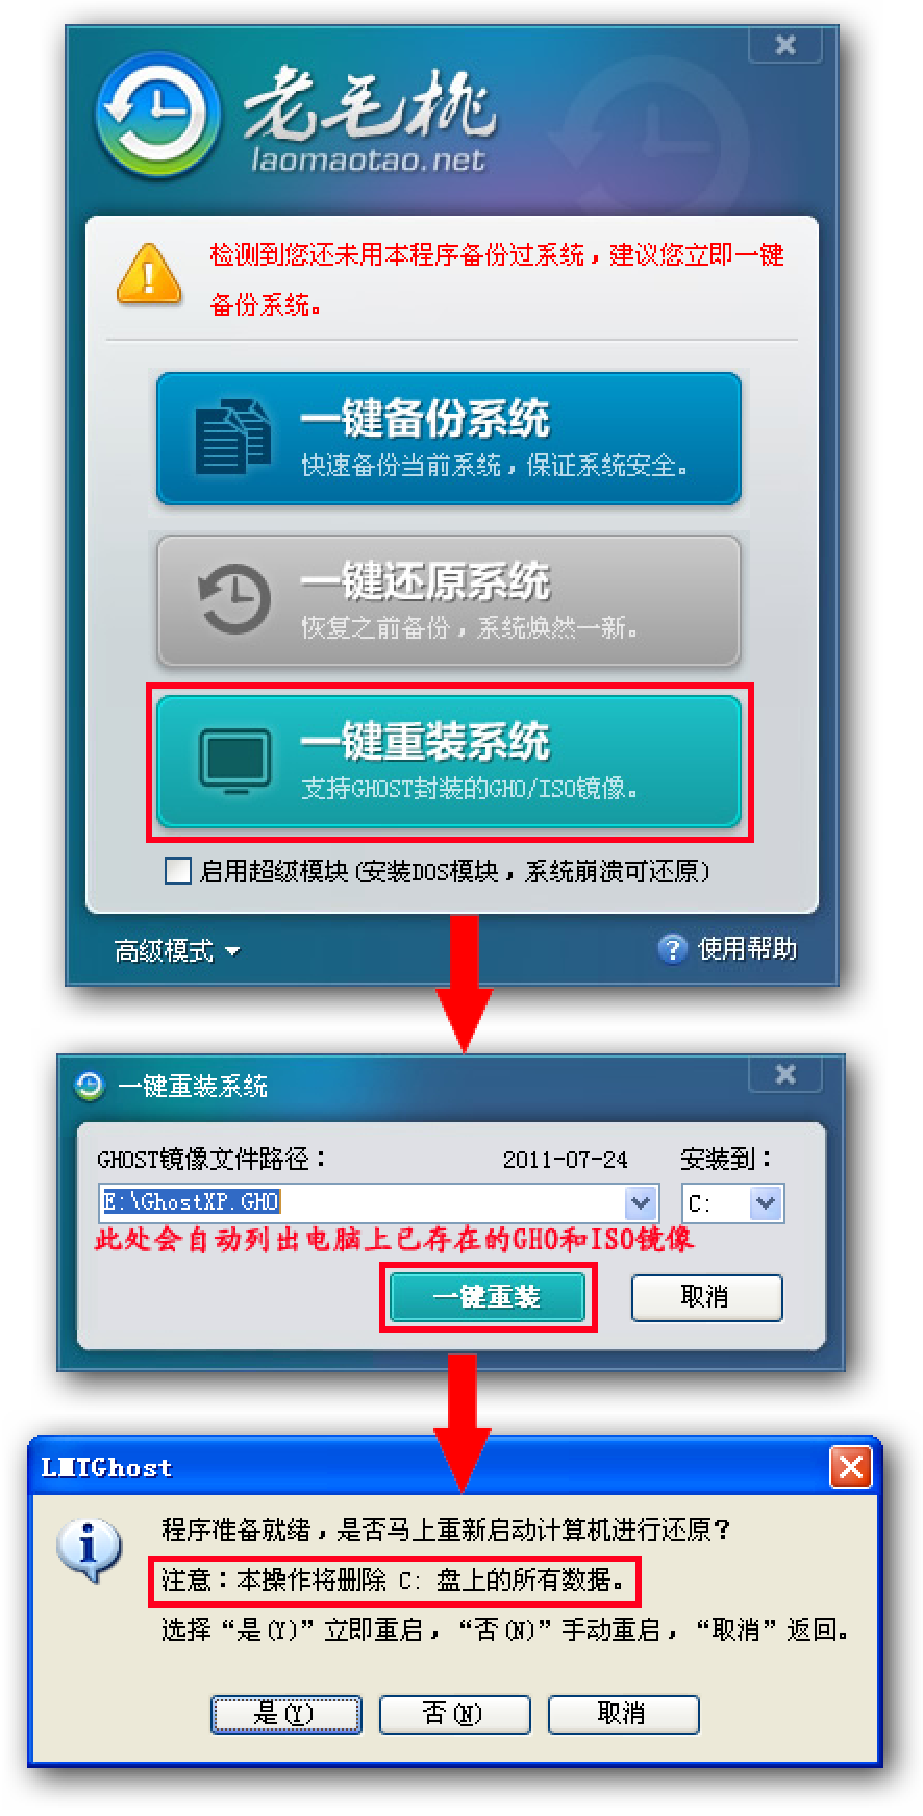
\includegraphics[scale=0.35]{figs/win_lmt_reinstall_startup.pdf}
    	\label{fig:win_lmt_backup_result}
\end{figure}
\end{enumerate}

\end{itemize}
\clearpage
\section{编程开发}
\clearpage
\section{其他软件}
\subsection{ubuntu one-网盘}
背景介绍\\

Ubuntu One是由Ubuntu背后的公司Canonical所推出的一项网络服务。该服务能够存储你的文件,并允许你在多台电脑上同步,还可以与好友分享这些文件。\\
准备工作
\begin{itemize}
\item 帐号--\href{https://one.ubuntu.com/dashboard}{ubuntu one官网}
\item 软件--\href{https://one.ubuntu.com/downloads/windows/}{Ubuntu One}
\end{itemize} 
优势总结
\begin{description}
\item[跨平台] 目前的客户端支持windows,ubuntu,mac,android和iphone
\item[容量] 免费5G,\$2.99/月即可获得20G。
\item[速度] 同步速度大约在80kb/s,更重要的是同步响应非常快。
\item[共享] 指定欲分享用户的Email地址既可分享文件夹,发送链接既可分享指定文件。
\end{description}
使用推荐:\textcolor{red}{存储私人关键文件}

\subsection{google driver-网盘}
背景介绍\\

Google Drive,美国谷歌公司于2012年4月24日正式推出的一项云存储服务,可以向用户提供5GB的免费存储空间,同时还可以付费扩容。\\
准备工作
\begin{itemize}
\item google帐号--\href{https://accounts.google.com/SignUp?hl=zh-CN}{帐号注册}
\item 软件--\href{http://drive.google.com}{云端硬盘}
\end{itemize} 
优势总结
\begin{description}
\item[跨平台] 目前的客户端支持windows,mac,android和ubuntu(有适用期)
\item[容量] 免费5G,\$2.49/月即可获得25G。
\item[在线浏览] 支持多达30多种文件的直接预览。
\item[集中管理] 对于文件的管理非常方便。
\end{description}
使用推荐:\textcolor{red}{作为公开网盘,用来存储文档以及常用软件}


\subsection{dropbox-网盘}
背景介绍\\

Dropbox是一个提供同步本地文件的网络存储在线应用。支持在多台电脑多种操作中自动同步。并可当作大容量的网络硬盘使用。\\
准备工作
\begin{itemize}
\item 帐号--\href{https://www.dropbox.com/}{dropbox官网}
\item 软件--\href{http://dropboxchina.com/Download/dropbox-for-windows.html}{dropbox}
\end{itemize} 
优势总结
\begin{description}
\item[跨平台] 目前的客户端支持windows,ubuntu,mac,android,iphone和blackberry
\item[容量] 免费3G,通过邀请朋友可获得额外空间。
\item[图片预览] 支持图片直接预览。
\item[国外流行] 成为很多软件首选的备份点,如springseed。
\end{description}
使用推荐:\textcolor{red}{配合android版备份手机上的照片}


\clearpage
\section{安全杀毒}
\clearpage















\part{Linux}
\setcounter{section}{0}
\clearpage
\section{压缩刻录}
\subsection{unetbootin-制作usb启动盘}
准备工作
\begin{itemize}
\item u盘
\item iso镜像文件--\href{http://releases.ubuntu.com/precise/}{ubuntu-12.04.2-desktop-amd64.iso}
\item 刻录软件--\href{http://www.oschina.net/news/9166/oschina-os-week-recommended-UNetbootin}{unetbootin-linux-583}
\end{itemize} 
操作步骤
\begin{enumerate}
\item 格式化u盘
\begin{itemize}
\item 查看u盘信息
\begin{lstlisting}[style=BASH]
hjy@jy:~$ mount
/dev/sdb1 on /media/KINGSTON type vfat (rw,nosuid,nodev,uid=1000,gid=1000,shortname=mixed,dmask=0077,utf8=1,showexec,flush,uhelper=udisks)
\end{lstlisting}

\item 卸载u盘
\begin{lstlisting}[style=BASH]
hjy@jy:~$ umount /media/KINGSTON
\end{lstlisting}

\item 格式化
\begin{lstlisting}[style=BASH]
hjy@jy:~$ mkfs -t vfat /dev/sdb1
\end{lstlisting}
\end{itemize}
\item 启动并设置unetbootin-linux-583参数\\
\begin{figure}[!htbp]
	\centering
	\caption{参数设置}  
		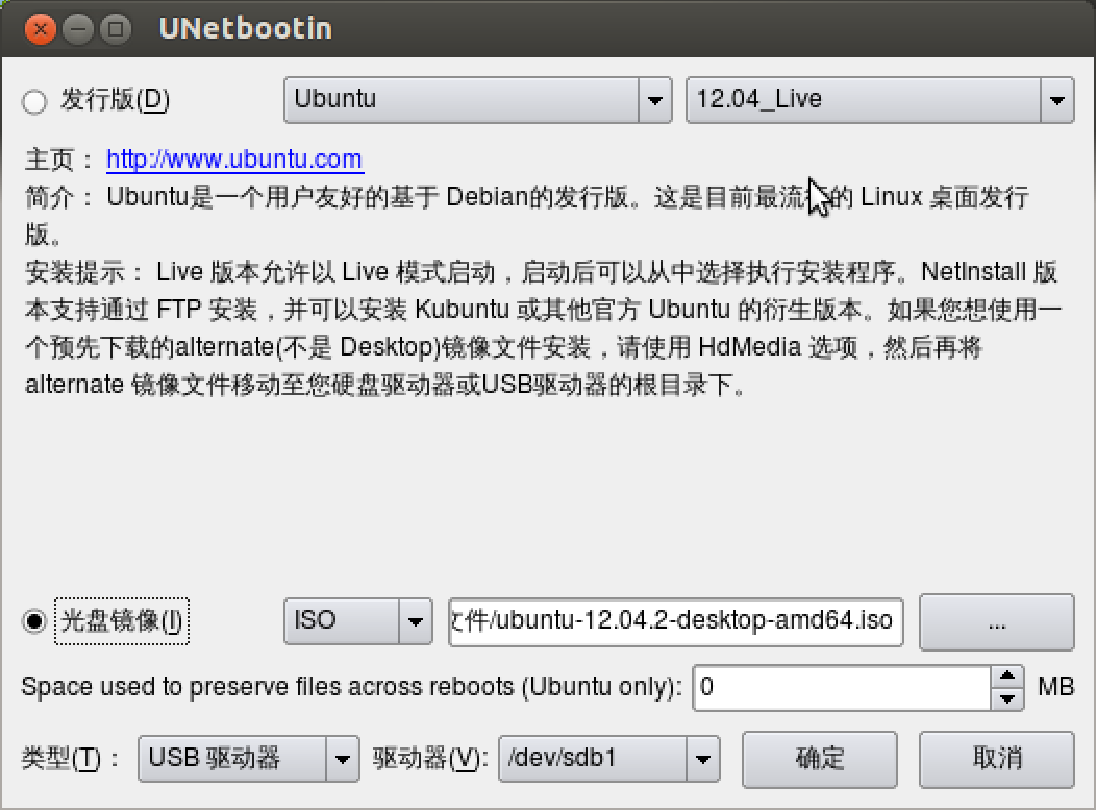
\includegraphics[scale=0.35]{figs/ubuntu_unetbootin_set.pdf}
    	\label{fig:unetbootin_set}
\end{figure}
注意:\textcolor{red}{软件能够识别u盘--u盘一定要插在电脑上}
\end{enumerate}
\textcolor{blue}{ubuntu安装命令:}
\begin{lstlisting}[style=BASH]
hjy@jy:~$ sudo apt-get install unetbootin
\end{lstlisting}

\clearpage
\section{聊天工具}
\section{视频软件}
\subsection{xbmc--包罗万象的媒体中心}
准备工作
\begin{itemize}
\item 插件--\href{}{xbmc中文插件.zip}
\end{itemize}

安装步骤:
\begin{enumerate}
\item 添加软件源
\begin{lstlisting}[style=BASH]
hjy@jy:~$ sudo add-apt-repository ppa:team-xbmc/ppa
\end{lstlisting}

\item 更新软件源
\begin{lstlisting}[style=BASH]
hjy@jy:~$ sudo apt-get update
\end{lstlisting}

\item 安装软件
\item 更新软件源
\begin{lstlisting}[style=BASH]
hjy@jy:~$ sudo apt-get install xbmc
\end{lstlisting}
\end{enumerate}
软件配置:
\begin{itemize}
\item 汉化
\begin{enumerate}
\item System$\rightarrow{}$appearance$\rightarrow{}$Skin$\rightarrow{}$Arial based\textcolor{red}{(必须先设置)}
\item International$\rightarrow{}$Chinese(simple),Character Set$\rightarrow{}$Chinese Simplified
\end{enumerate}
\item 插件
\begin{enumerate}
\item 解压出repository.googlecode.xbmc-addons-chinese.zip\textcolor{red}{(就是zip格式)}
\item 系统设置$\rightarrow{}$扩展功能$\rightarrow{}$从zip中安装
\item 从扩展功能里面选择获取扩展功能,点全部扩展功能
\begin{itemize}
\item 视频插件
\begin{itemize}
\item 迅雷看看(KanKan)
\item PPTV视频
\item 酷狗MV(KugouMV)
\item 乐视网(LeTV)
\item 优酷视频(YouKu)
\item PPS网络电视(PPStream)
\item 中国网络电视台点播(CNTV)
\item 音悦台MV(YinYueTai)
\item 土豆视频(Tudou)
\item 奇艺视频(QIYI)
\item 腾讯视频(Tecent)
\item 新浪视频(Sina)
\end{itemize}
\item 音频插件
\begin{itemize}
\item KuwoBox/酷我音乐盒插件
\item BaiduRadio/百度电台联盟插件
\item TOP100/巨鲸音乐网插件
\end{itemize}
\item 字幕
\begin{itemize}
\item LRC同步歌词脚本
\item shooterSub/射手字幕脚本
\end{itemize}
\item 天气
\begin{itemize}
\item 中国天气(Weather China)
\end{itemize}
\end{itemize}
\end{enumerate}
\end{itemize}





\clearpage
\section{音乐软件}
\section{游戏软件}
\section{网络游戏}
\section{浏览器}
\section{图形图像}
\section{输入法}
\section{下载工具}
\section{办公软件}
\subsection{latex(包括中文环境)}
\subsubsection{精简版}

\begin{itemize}
\item 安装texlive-latex-base:基本核心包
\begin{lstlisting}[style=BASH]
hjy@jy:~$ sudo apt-get install texlive-latex-base
\end{lstlisting}
\item 安装latex-cjk-all:中文环境需要的包
\begin{lstlisting}[style=BASH]
hjy@jy:~$ sudo apt-get install texlive-cjk-all
\end{lstlisting}
\item 安装texlive-latex-extra:一些常用的包文件
\begin{lstlisting}[style=BASH]
hjy@jy:~$ sudo apt-get install texlive-latex-extra
\end{lstlisting}
\item 安装texmaker:latex文档编辑器
\begin{lstlisting}[style=BASH]
hjy@jy:~$ sudo apt-get install texmaker
\end{lstlisting}
\end{itemize}

注意:\textcolor{red}{有些.sty文件可能没有安装,如lastpage.sty.可按下面的命令来查找相应的包}
\begin{lstlisting}[style=BASH]
hjy@jy:~$ apt-cache search lastpage
\end{lstlisting}

\subsubsection{完整版}

\begin{itemize}
\item 安装texlive-full:texlive完整包
\begin{lstlisting}[style=BASH]
hjy@jy:~$ sudo apt-get install texlive-full
\end{lstlisting}
\item 安装texmaker:latex文档编辑器
\begin{lstlisting}[style=BASH]
hjy@jy:~$ sudo apt-get install texmaker
\end{lstlisting}
\end{itemize}
注意:\textcolor{red}{完整包比较大,下载可能需要不少时间}

\subsubsection{\href{http://blog.csdn.net/sdupine/article/details/7958668}{添加utf8字体}}

\begin{itemize}
\item 首先要生成Tex用户个人配置,使用Tex的updmap 命令
\begin{lstlisting}[style=BASH]
hjy@jy:~$ updmap
hjy@jy:~$ sudo update-updmap
hjy@jy:~$ updmap
\end{lstlisting}
\textcolor{red}{Latex默认的用户配置文件位于Home下的.texmf-var [~/.texmf-var]目录中,请检查命令给出的信息,确定目录,后面会使用。}
\item 给Tex用户个人配置目录添加读写权限
\begin{lstlisting}[style=BASH]
hjy@jy:~$ sudo chmod -R 777 .texmf-var
\end{lstlisting}
\item 修改mkfont文件夹中的mkfont.sh文件\\
将第四行修改为:
\begin{lstlisting}[style=BASH]
TEXMF=~/.texmf-var
\end{lstlisting}
\textcolor{red}{mkfont文件夹中mkfont.sh文件中已经做过修改,要是用mkfont.tar中的文件则还要进行其它修改}
\item 把字体文件拷贝到 mkfont 目录中,并执行命令
\begin{lstlisting}[style=BASH]
hjy@jy:~$ ./mkfont.sh fontName.ttf fontName fontShortName
\end{lstlisting}
\item 测试结果如图\ref{fig:latex_fonts}
\begin{figure}[!htbp]
	\centering
	\caption{基本设置}  
		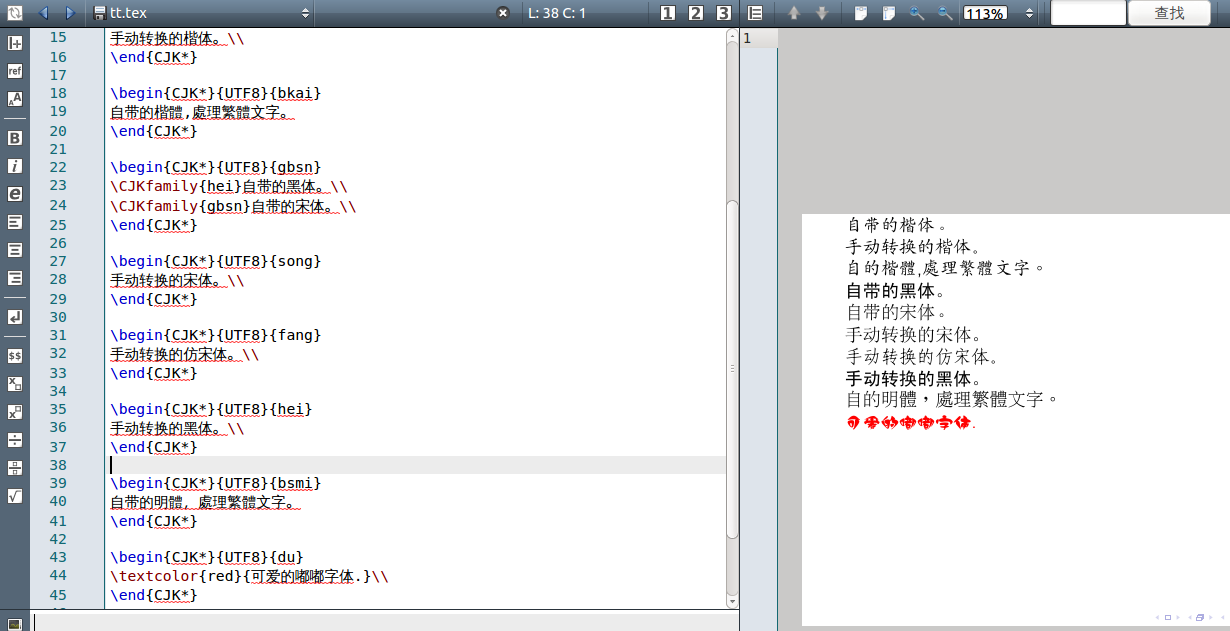
\includegraphics[scale=0.25]{figs/ubuntu_latex_fonts.png}
    	\label{fig:latex_fonts}
\end{figure}
\end{itemize}




\subsection{blogilo}
blogilo是linux下面一款开源的写博客的客户端,可以写博客园以及wordpress的博客,与windows下面的windows live有的一拼。安装命令如下:
\begin{lstlisting}[style=BASH]
hjy@jy:~$ sudo apt-get install blogilo
\end{lstlisting}

软件配置:
\begin{enumerate}
\item 博客$\rightarrow{}$添加博客,得到下图\ref{fig:blogilo_base}:
\begin{figure}[!htbp]
	\centering
	\caption{基本设置}  
		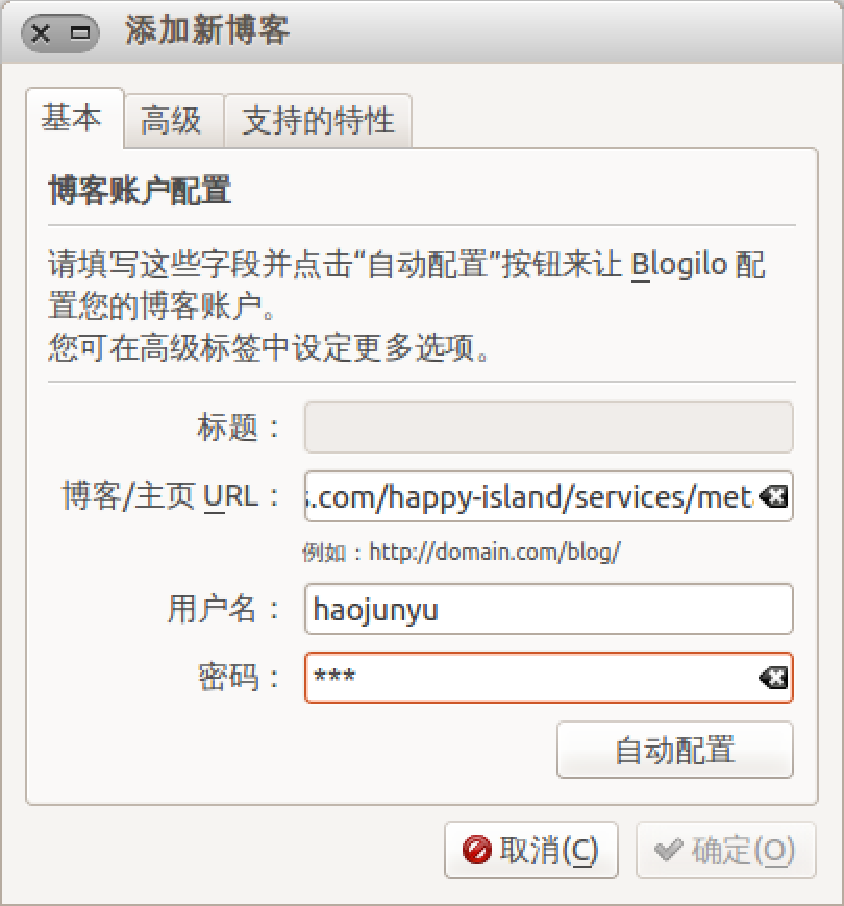
\includegraphics[scale=0.25]{figs/ubuntu_blogilo_base.pdf}
    	\label{fig:blogilo_base}
\end{figure}
在URL里输入你的博客地址,格式为“\textcolor{red}{http://www.cnblogs.com/Blog名/services/metaweblog.aspx}”,然后再输入用户名和密码。

\item 点击上图中“高级”页面,选择API为“MetaWeblog API”,然后点击“获取ID”,即可得到下图\ref{fig:blogilo_advantage}:
\begin{figure}[!htbp]
	\centering
	\caption{高级设置}  
		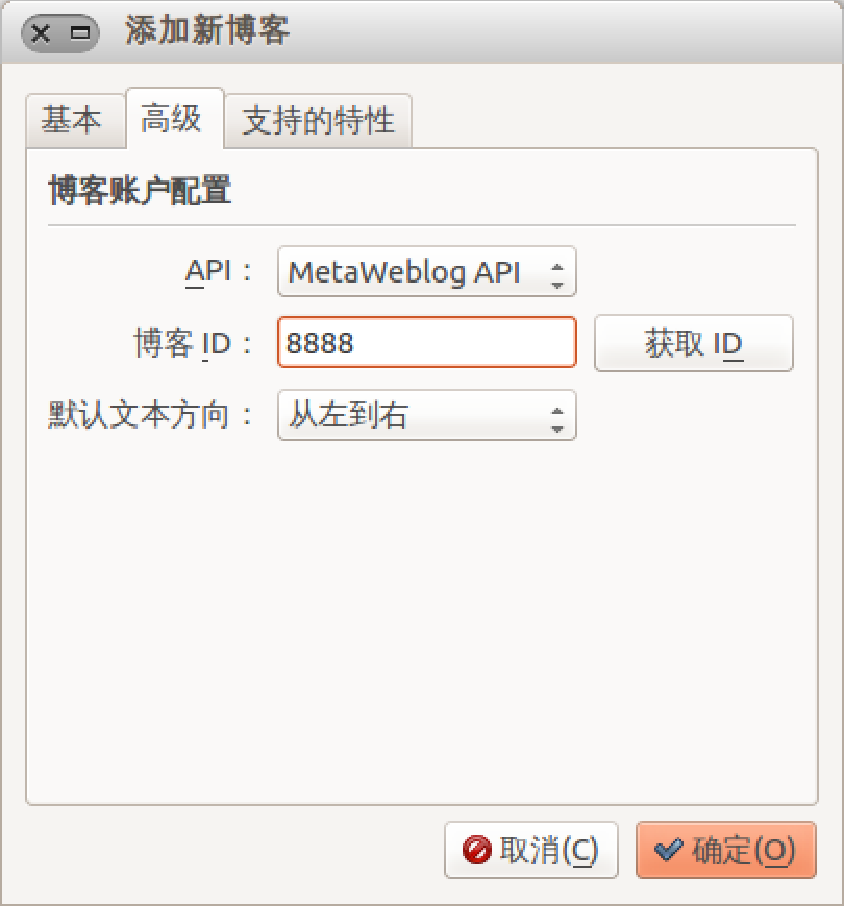
\includegraphics[scale=0.25]{figs/ubuntu_blogilo_advantage.pdf}
    	\label{fig:blogilo_advantage}
\end{figure}

\item 单击确定,大功告成。

\end{enumerate}




\clearpage
\section{阅读翻译}
\section{系统工具}
\section{编程开发}
\subsection{matlab2011a}
准备工作\\
\begin{itemize}
\item iso镜像文件--\href{http://url.cn/Ius1xq}{Matlab.R2011a.UNIX.ISO-TBE.iso}
\item 创建挂载目录,并挂载iso文件到该目录(文件在桌面上)
\begin{lstlisting}[style=BASH]
hjy@jy:~$ sudo mkdir /mnt/iso
hjy@jy:~$ sudo mount -o loop 桌面/Matlab.R2011a.UNIX.ISO-TBE.iso /mnt/iso
\end{lstlisting}
\end{itemize} 
安装步骤\\
\begin{itemize}
\item 变更目录,并运行install进入图形安装
\begin{lstlisting}[style=BASH]
hjy@jy:~$ cd /mnt/iso
hjy@jy:~$ sudo ./install
\end{lstlisting}
\item 选择"install manually without using the internet"
\item accept the terms of the license agreement,选择“yes”
\item 选择I have the File Installation Key for my license:$59327-00840-06743-08309-05690$(standalone模式)或$31996-44762-21423-39948-52406$(network模式)
\item 选择Typical(典型安装)
\item 安装到指定目录/opt/matlab(默认会安装到/usr/local/MATLAB/R2011b文件夹中)
\item 等待、安装...
\item 激活--将crack文件夹复制到安装目录/opt/matlab
\begin{lstlisting}[style=BASH]
hjy@jy:~$ sudo cp -r crack /opt/matlab
\end{lstlisting}
若选择standalone模式,则选择"/opt/matlab/crack/license\_{}standalone.dat"文件。\\
若选择network模式,则选择"/opt/matlab/crack/license\_{}server.dat"文件。\\
\end{itemize} 

\textcolor{red}{常见问题:}
\begin{enumerate}
\item 直接输入matlab无法启动
\begin{lstlisting}[style=BASH]
hjy@jy:~$ sudo ln -s /opt/matlab/bin/matlab /usr/bin/matlab
\end{lstlisting}

\item 创建桌面启动图标
通过“启动应用程序”创建matlab.desktop。注意启动命令为\textcolor{red}{/opt/matlab/bin/matlab -desktop}

\item 在终端下运行matlab出现 /lib64/libc.so.6: not found
\begin{lstlisting}[style=BASH]
hjy@jy:~$ sudo ln -s /lib/x86_64-linux-gnu/libc.so.6 /lib64/libc.so.6
\end{lstlisting}

\item matlab下中文无法显示(中文显示方框框)
打开matlab,file->Preference->Fonts,在Desktop code font和Desktoop text font选择下拉菜单。最后面有一些无法显示名字的字体,选择它们,点击Apply就可以显示中文
\end{enumerate}


\subsection{github}
Git是一个免费的、分布式的版本控制工具,或是一个强调了速度快的源代码管理工具。每一个Git的工作目录都是一个完全独立的代码库,并拥有完整的历史记录和版本追踪能力,不依赖于网络和中心服务器。其代码状态转换图如图\ref{fig:ubuntu_git_flow}所示:
\begin{figure}[!htbp]
	\centering
	\caption{git工作状态转换图}  
		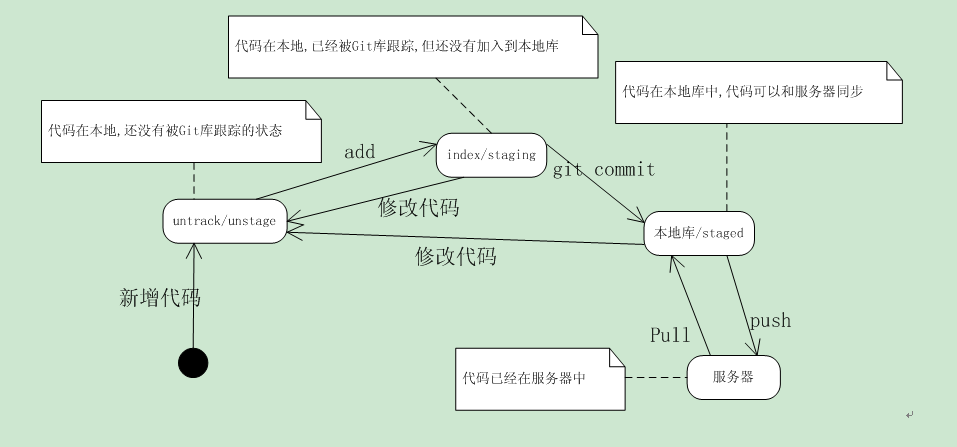
\includegraphics[scale=0.40]{figs/ubuntu_git_flow.png}
    	\label{fig:ubuntu_git_flow}
\end{figure}\\
其中各个状态注释如下:
\begin{enumerate}
\item 未被Git跟踪的状态为unstage状态,包括两种情况
\begin{itemize}
\item untrack files是指尚未被git所管理的文件
\item changed but not updated是指文件被git管理,并且发生了改变,但改动还没被git管理
\end{itemize}
\item 已经被Git跟踪的状态为stage状态,因此包括staging状态和staged状态
\item changes to be commited是指进入stage状态的文件,stage是commit和未管理之间的一个状态,也有别名叫index状态,也就是git已经管理了这些改动,但是还没完成提交。
\item .gitignore中的文件,不会出现在以上三个状态中。
\end{enumerate}

安装Git客户端如下:
\begin{lstlisting}[style=BASH]
hjy@jy:~$ sudo apt-get install git
\end{lstlisting}

软件配置:
\begin{enumerate}
\item 在https://github.com/注册一个账户(代码是托管在GitHub上),创建一个repository(ParallelComputation),SSH Keys$\rightarrow{}$ADD SSH key
\item 创建公钥
\begin{lstlisting}[style=BASH]
hjy@jy:~$ ssh-keygen -C "haojunyu2012@gmail.com" -f ~/.ssh/github
\end{lstlisting}
\item 将~/.ssh/github.pub文件中的内容复制到key中,并起一个tittle。
\item 验证方法
\begin{lstlisting}[style=BASH]
hjy@jy:~$ ssh -T git@github.com
Hi haojunyu! You've successfully authenticated, but GitHub does not provide shell access.
\end{lstlisting}
\item 设置git全局环境并查看
\begin{lstlisting}[style=BASH]
hjy@jy:~$ git config --global user.name "haojunyu"
hjy@jy:~$ git config --global user.email "haojunyu2012@gmail.com"
hjy@jy:~$ git config --list
\end{lstlisting}
\item 从服务器下载代码,准确的说应该是从GitHub服务器复制一个版本库到本地
\begin{lstlisting}[style=BASH]
hjy@jy:~$ mkdir git
hjy@jy:~$ cd git
hjy@jy:~$ git clone git@github.com:haojunyu/ParallelComputation.git
\end{lstlisting}
\item 获取到源码之后,就可以进行开发了,代码开发完成就可以提交代码
\begin{lstlisting}[style=BASH]
hjy@jy:~$ git add . 	// 往暂存区域添加已添加和修改的文件,不处理删除的文件
hjy@jy:~$ git status	// 比较本地数据目录与暂存区域的变化	
hjy@jy:~$ git commit -m "commit directions"	// 提到代码到本地数据目录,并添加提交说明
\end{lstlisting}
\item 有可能你和其他人改的是同一个文件,那么冲突的情况是在所难免的,那么在提交之后再获取一下代码,就会提示代码冲突的文件,我们需要做的就是处理这些冲突,并再次提交
\begin{lstlisting}[style=BASH]
hjy@jy:~$ git pull	// 更新代码
hjy@jy:~$ git status	
hjy@jy:~$ git commit -m "commit directions"	
\end{lstlisting}
\item 当你做完以上的步骤的时候,你需要做的是把本地数据目录的版本库的数据同步到GitHub服务器上去,这样你的同事才能够看到你作出的修改
\begin{lstlisting}[style=BASH]
hjy@jy:~$ git remote add ParaComp git@github.com:haojunyu/ParallelComputation.git	// 给仓库命名
hjy@jy:~$ git push ParaComp master		// 同步到服务器上
\end{lstlisting}

\end{enumerate}


\subsection{opengl}
OpenGL(全写Open Graphics Library)是个定义了一个跨编程语言、跨平台的编程接口的规格,它用于三维图象(二维的亦可)。OpenGL是个专业的图形程序接口,是一个功能强大,调用方便的底层图形库。

ubuntu配置opengl如下:
\begin{enumerate}
\item 安装编译环境
\begin{lstlisting}[style=BASH]
hjy@jy:~$ sudo apt-get install build-essential
\end{lstlisting}

\item 安装OpenGL Utilities
\begin{lstlisting}[style=BASH]
hjy@jy:~$ sudo apt-get install libgl1-mesa-dev
\end{lstlisting}

\item 安装OpenGL Utilities\\
一组建构于 OpenGL Library 之上的工具组,提供许多很方便的函式,使 OpenGL 更强大且更容易使用。
\begin{lstlisting}[style=BASH]
hjy@jy:~$ sudo apt-get install libgl1-mesa-dev
\end{lstlisting}

\item 安装OpenGL Utility Toolkit\\
建立在 OpenGL Utilities 上面的工具箱,除了强化了 OpenGL Utilities 的不足之外,也增加了 OpenGL 对于视窗介面支援。
\begin{lstlisting}[style=BASH]
hjy@jy:~$ sudo apt-get install freeglut3-dev
\end{lstlisting}

\end{enumerate}


\clearpage
\section{其他软件}
\subsection{ubuntu one-网盘}
背景介绍\\

Ubuntu One是由Ubuntu背后的公司Canonical所推出的一项网络服务。该服务能够存储你的文件,并允许你在多台电脑上同步,还可以与好友分享这些文件。\\
准备工作
\begin{itemize}
\item 帐号--\href{https://one.ubuntu.com/dashboard}{ubuntu one官网}
\item ubuntu系统自带软件--\href{https://one.ubuntu.com/downloads/ubuntu}{Ubuntu One}
\end{itemize} 
优势总结
\begin{description}
\item[跨平台] 目前的客户端支持windows,ubuntu,mac,android和iphone
\item[容量] 免费5G,\$2.99/月即可获得20G。
\item[速度] 同步速度大约在80kb/s,更重要的是同步响应非常快。
\item[共享] 指定欲分享用户的Email地址既可分享文件夹,发送链接既可分享指定文件。
\end{description}
使用推荐:\textcolor{red}{存储私人关键文件}

\subsection{google driver-网盘}
背景介绍\\

Google Drive,美国谷歌公司于2012年4月24日正式推出的一项云存储服务,可以向用户提供5GB的免费存储空间,同时还可以付费扩容。\\
准备工作
\begin{itemize}
\item google帐号--\href{https://accounts.google.com/SignUp?hl=zh-CN}{帐号注册}
\item ubuntu软件--\href{https://www.insynchq.com/linux}{insync}
\end{itemize} 
优势总结
\begin{description}
\item[跨平台] 目前的客户端支持windows,mac,android和ubuntu(有适用期)
\item[容量] 免费5G,\$2.49/月即可获得25G。
\item[在线浏览] 支持多达30多种文件的直接预览。
\item[集中管理] 对于文件的管理非常方便。
\end{description}
使用推荐:\textcolor{red}{作为公开网盘,用来存储文档以及常用软件}


\subsection{dropbox-网盘}
背景介绍\\

Dropbox是一个提供同步本地文件的网络存储在线应用。支持在多台电脑多种操作中自动同步。并可当作大容量的网络硬盘使用。\\
准备工作
\begin{itemize}
\item 帐号--\href{https://www.dropbox.com/}{dropbox官网}
\item 软件--ubuntu软件中心/\href{https://www.dropbox.com/install2}{dropbox}
\end{itemize} 
优势总结
\begin{description}
\item[跨平台] 目前的客户端支持windows,ubuntu,mac,android,iphone和blackberry
\item[容量] 免费3G,通过邀请朋友可获得额外空间。
\item[图片预览] 支持图片直接预览。
\item[国外流行] 成为很多软件首选的备份点,如springseed。
\end{description}
使用推荐:\textcolor{red}{配合android版备份手机上的照片}


\clearpage
\section{安全杀毒}

















\clearpage     
\end{CJK*}
\end{document}
\part{常见错误}
%Frequently Asked Questions
\section{boot分区剩余空间不足}
\begin{description}
\item[问题] \textcolor{red}{boot分区剩余空间不足}\\
\begin{figure}[!htbp]
	\centering
	\caption{boot分区剩余空间不足}  
		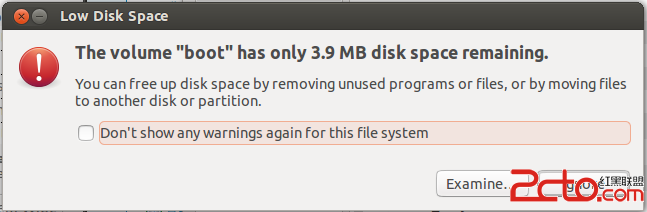
\includegraphics[scale=0.35]{figs/boot_space.png}
    	\label{fig:boot_space}
\end{figure}
\item[原因] \textcolor{blue}{
boot分区里面存放的是系统引导文件和内核的一些东西,这些东西100M是足够容纳的。而大家都知道linux内核一直在更新,跟新后,旧的内核就不在使用,但旧的内核文件还在boot里面,占据着空间,更新几次过后boot文件就会被占满,显示boot磁盘空间不足。这时为了更新需要将不用的内核文件删除,释放空间。
}
\item[方案]
\begin{enumerate}
\item 查看已安装的linux-image各版本\\
\begin{lstlisting}[style=BASH]
hjy@jy:~$ dpkg --get-selections | grep linux-image
\end{lstlisting}

\item 查看当前正在使用的镜像版本\\
\begin{lstlisting}[style=BASH]
hjy@jy:~$ uname -a
\end{lstlisting}

\item 卸载老版本\textcolor{red}{建议保留最新的两个版本}
\begin{lstlisting}[style=BASH]
hjy@jy:~$ sudo apt-get purge linux-image-3.x.x-xx-generic
\end{lstlisting}

\end{enumerate}

\end{description}


\clearpage     
\end{CJK*}
\end{document}